\documentclass[11pt,a4paper]{article}

% --- Language, Encoding, and Fonts ---
\usepackage[utf8]{inputenc}
\usepackage[T1]{fontenc}
\usepackage[english]{babel}
\usepackage{lmodern}

% --- Mathematics and Symbols ---
\usepackage{amsmath, amssymb, amsfonts, mathtools}

% --- Page Layout ---
\usepackage[top=2.2cm, bottom=2.2cm, left=2.2cm, right=2.2cm]{geometry}
\usepackage{microtype}
\usepackage{setspace}
\setstretch{1.08}

% --- Figures, Subfigures, and Tables ---
\usepackage{graphicx}
\graphicspath{{./}{../}{figures/}{../figures/}}
\usepackage{subcaption}
\usepackage{float}
\usepackage{booktabs}
\usepackage{array}
\usepackage{multirow}

% --- Code Listings ---
\usepackage{listings}
\usepackage{xcolor}

\definecolor{codegreen}{rgb}{0,0.6,0}
\definecolor{codegray}{rgb}{0.45,0.45,0.45}
\definecolor{codepurple}{rgb}{0.55,0,0.8}
\definecolor{backcolour}{rgb}{0.97,0.97,0.98}

\lstdefinestyle{codeStyle}{
    backgroundcolor=\color{backcolour},   
    commentstyle=\color{codegreen}\itshape,
    keywordstyle=\color{blue}\bfseries,
    numberstyle=\tiny\color{codegray},
    stringstyle=\color{codepurple},
    basicstyle=\ttfamily\footnotesize,
    breakatwhitespace=false,         
    breaklines=true,                 
    captionpos=b,                    
    keepspaces=true,                 
    numbers=left,                    
    numbersep=5pt,                  
    showspaces=false,                
    showstringspaces=false,
    showtabs=false,                  
    tabsize=2,
    frame=single,
    rulecolor=\color{lightgray}
}
\lstset{style=codeStyle}

% --- Hyperlinks & Bibliography ---
\usepackage[colorlinks=true, linkcolor=blue, urlcolor=blue, citecolor=blue]{hyperref}
\usepackage{cite}

% ========================================================
% TITLE & AUTHOR METADATA
% ========================================================
\title{
    \vspace{-1.0cm}
    \textbf{\Large Sub-Pixel Registration and Deep Residual Contrast Refinement for Temporal Dental Radiography: A Multi-Scale Dilated Convolutional Approach}
}

\author{
    \textbf{İpek Koçhisarlı} \\[0.2cm]
    \small Department of Computer Engineering, Graduate School of Natural and Applied Sciences \\
    \small Ege University, İzmir, Turkey \\
    \small \texttt{ipekkochisarli@gmail.com}
}

\date{\small Academic Research Report $\cdot$ November 2026}

\begin{document}

\maketitle
\thispagestyle{empty}

% ========================================================
% ABSTRACT
% ========================================================
\begin{abstract}
\noindent Digital subtraction radiography (DSR) is a critical diagnostic modality for assessing longitudinal alveolar bone loss, periodontal progression, and endodontic therapy efficacy. However, subtle patient motion, projection geometry variations, tube angulation shifts, and X-ray beam scatter induce pronounced spatial and photometric misalignments that corrupt subtraction images. In this paper, we propose a rigorous, two-stage registration and residual refinement framework tailored for periapical dental radiographs. In the first stage, we conduct a systematic benchmark comparing six geometric transformation families (Similarity, Affine, Projective, 2nd-degree Polynomial, Piecewise Linear, and Local Weighted Mean) across three interpolation schemes (Nearest, Bilinear, Bicubic) guided by 64 anatomically curated dental landmarks. In the second stage, to overcome the intrinsic limits of spatial warping and compensate for complex scattered-radiation residuals without corrupting delicate dental morphology, we develop a novel \textbf{Multi-Scale Dilated Residual Network (MDRN)}. Operating without pooling layers, MDRN combines parallel dilated convolutions ($d \in \{1, 2, 4\}$) with a bounded residual mapping mechanism and a composite objective coupling robust Charbonnier loss with Sobel gradient edge preservation. Extensive evaluations demonstrate that our framework elevates radiograph alignment from an initial baseline of $15.48\text{ dB}$ ($MSE = 1843.8$) to $32.27\text{ dB}$ via optimal landmark registration, and culminates at \textbf{36.66 dB} ($MSE = 14.02$) through MDRN refinement. This represents a cumulative quantitative gain of \textbf{+21.18 dB}, substantially outperforming standard two-layer residual CNNs while preserving critical periodontal enamel and pulp canal boundaries.
\end{abstract}

\vspace{0.3cm}
\noindent\textbf{Keywords:} Medical Image Registration, Dental Radiography, Digital Subtraction Radiography, Multi-Scale Dilated Convolutions, Residual Networks, Charbonnier Loss.

\vspace{0.4cm}
\tableofcontents
\newpage

% ========================================================
% SECTION 1: INTRODUCTION
% ========================================================
\section{Introduction}
\label{sec:intro}

Periapical radiographs are among the most frequently utilized diagnostic imaging modalities in modern clinical dentistry. They provide high-resolution visualizations of crowns, root structures, pulp chambers, and surrounding trabecular alveolar bone tissue \cite{lehmann2000subtraction}. In longitudinal treatment monitoring—such as assessing periapical lesion healing, quantifying sub-millimeter marginal bone resorption in periodontitis, or tracking root canal therapy—clinicians frequently acquire temporal image pairs separated by weeks, months, or years \cite{zitova2003image, maintz1998survey}.

\textit{Digital Subtraction Radiography (DSR)} is an established diagnostic technique wherein an aligned baseline image is subtracted pixel-by-pixel from a follow-up image. When the radiographs are perfectly registered in both geometric space and intensity distribution, non-changing anatomical structures (e.g., sound enamel, dentin, baseline trabeculae) cancel out completely to zero, highlighting only genuine pathological changes as high-contrast intensity variations.

Despite its diagnostic potential, the clinical feasibility of DSR is severely impeded by three physical and radiological factors:
\begin{enumerate}
    \item \textbf{Geometric Misalignment:} Variations in X-ray tube angulation, sensor positioning inside the oral cavity, and patient head rotation introduce complex projective and non-rigid geometric transformations \cite{ostuni1997review, goshtasby1988image}.
    \item \textbf{Photometric and Exposure Discrepancies:} Differences in exposure time, tube voltage, developer chemistry, or digital sensor calibration produce global and localized contrast shifts.
    \item \textbf{High-Frequency Background Noise and Trabecular Scatter:} The porous, spongy architecture of trabecular bone introduces dense high-frequency textures that readily deceive intensity-based automated optimizers, frequently driving them into suboptimal local minima \cite{balakrishnan2019voxelmorph}.
\end{enumerate}

To resolve these challenges, this study presents an end-to-end medical vision pipeline that bridges classical spatial transformations and modern deep learning. We curate a set of 64 anatomical landmark pairs localized exclusively on tooth structures (completely omitting noisy trabecular bone), systematically benchmark 18 combinations of spatial transformations and interpolation schemes, and introduce a \textbf{Multi-Scale Dilated Residual Network (MDRN)} designed specifically for sub-pixel radiograph residual refinement.

% ========================================================
% SECTION 2: CLASSICAL PREPROCESSING & PHOTOMETRIC ALIGNMENT
% ========================================================
\section{Preprocessing and Photometric Alignment}
\label{sec:preprocessing}

\subsection{Region of Interest (ROI) Isolation}
Raw dental radiographs frequently contain non-anatomical peripheral artifacts, including rounded sensor margins, film-holder brackets, and large zero-padded borders. If retained, these artificial zero-intensity boundaries dominate histogram statistics, distort cumulative distribution calculations, and attract automated registration algorithms away from authentic tooth boundaries.

To eliminate these artifacts, we establish a synchronized bounding box covering two mandibular molar teeth, capturing the complete crowns, pulp chambers, root canals, apical foramina, and proximal alveolar bone crests. Let $I_{raw} \in \mathbb{R}^{H \times W}$ denote the original radiograph; the ROI extraction is formulated as:
\begin{equation}
    I_{roi}(x, y) = I_{raw}(x + x_0, \, y + y_0), \quad \forall \, 0 \le x < W_{roi}, \, 0 \le y < H_{roi}
\end{equation}
where $[x_0, y_0, W_{roi}, H_{roi}] = [85, 2, 351, 363]$, yielding uniform ROI dimensions of $364 \times 352$ pixels for both the reference ($I_{ref}$) and moving test ($I_{test}$) images (Figure~\ref{fig:roi_results}).

\begin{figure}[H]
    \centering
    \begin{subfigure}[b]{0.45\textwidth}
        \centering
        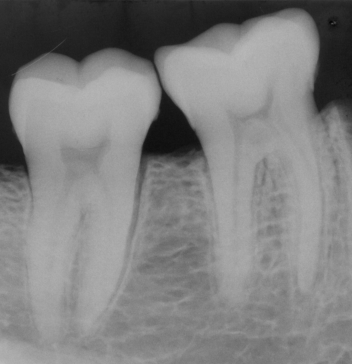
\includegraphics[width=0.82\textwidth]{figures/ref_roi.png}
        \caption{Reference ROI ($I_{ref}$)}
    \end{subfigure}
    \hfill
    \begin{subfigure}[b]{0.45\textwidth}
        \centering
        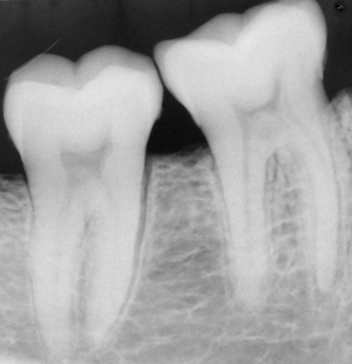
\includegraphics[width=0.82\textwidth]{figures/test_roi.png}
        \caption{Test ROI ($I_{test}$)}
    \end{subfigure}
    \caption{Extracted Regions of Interest (ROI) containing mandibular molars, free of sensor border artifacts.}
    \label{fig:roi_results}
\end{figure}

\subsection{Photometric Equalization via Histogram Matching}
As observed in Figure~\ref{fig:roi_results}, the test radiograph exhibits lower contrast and a lighter global intensity range due to lower radiation exposure. To equalize the photometric characteristics prior to geometric alignment, we apply global \textit{Histogram Matching} (Specification).

Let $r \in [0, 1]$ and $z \in [0, 1]$ represent continuous gray levels of the test and reference images, respectively. The Probability Density Functions (PDF) are denoted as $p_r(r)$ and $p_z(z)$. The respective Cumulative Distribution Functions (CDF) define the transformation mappings:
\begin{equation}
    s = T(r) = \int_{0}^{r} p_r(w) \, dw, \qquad v = G(z) = \int_{0}^{z} p_z(w) \, dw
\end{equation}
Because the reference transformation $G$ is monotonically increasing, the desired mapped level $\hat{z}$ is obtained via the inverse mapping:
\begin{equation}
    \hat{z} = G^{-1}(T(r))
\end{equation}
Figure~\ref{fig:contrast_comp} illustrates the contrast correction outcome, and Figure~\ref{fig:hist_curves} verifies that the cumulative distribution of the matched test radiograph coincides virtually identically with that of the reference image.

\begin{figure}[H]
    \centering
    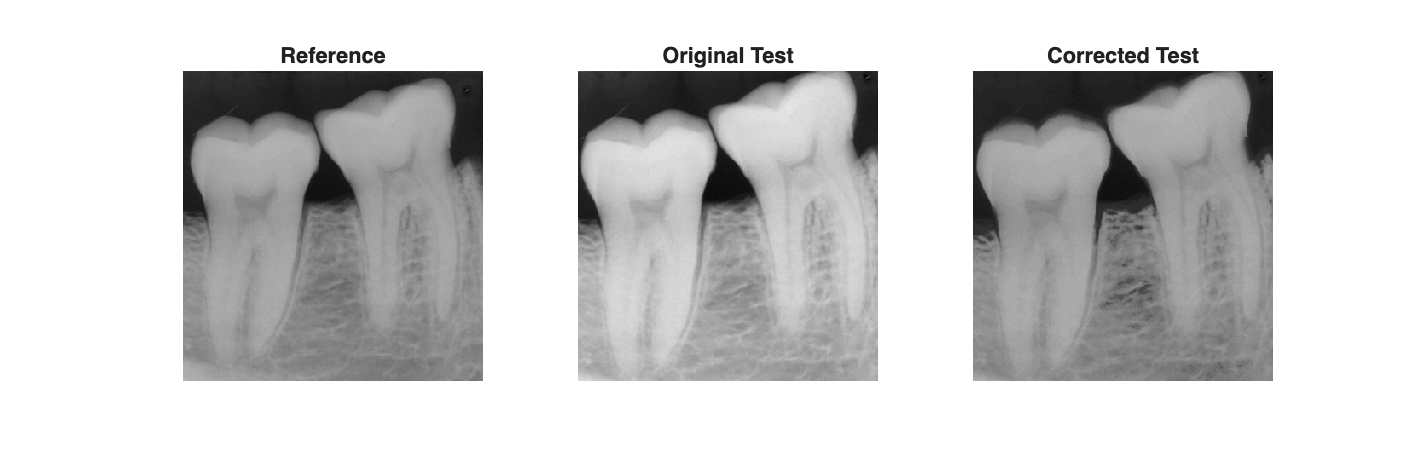
\includegraphics[width=0.88\textwidth]{figures/contrast_comparison.png}
    \caption{Contrast correction: Reference image, original test radiograph, and histogram-matched test radiograph.}
    \label{fig:contrast_comp}
\end{figure}

\begin{figure}[H]
    \centering
    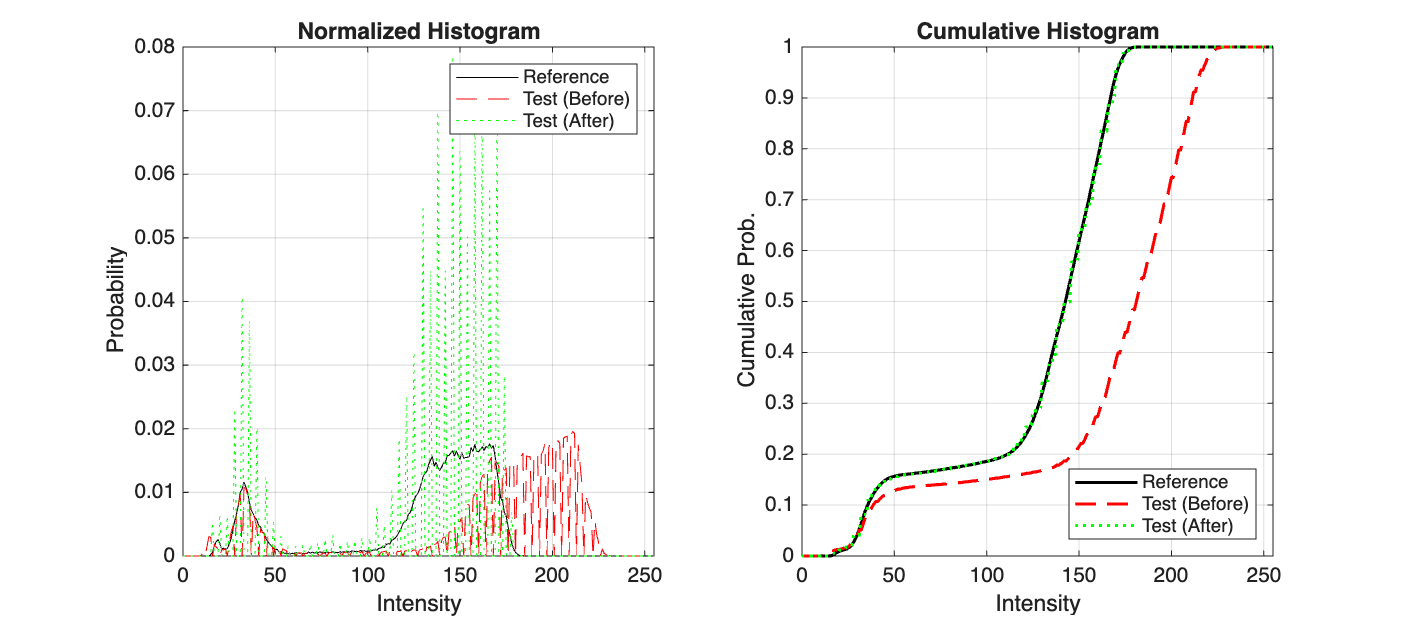
\includegraphics[width=0.80\textwidth]{figures/histogram_curves.png}
    \caption{Normalized probability density (PDF) and cumulative distribution (CDF) comparisons confirming successful photometric alignment.}
    \label{fig:hist_curves}
\end{figure}

% ========================================================
% SECTION 3: GEOMETRIC REGISTRATION BENCHMARK
% ========================================================
\section{Multi-Model Geometric Registration Benchmark}
\label{sec:registration}

\subsection{Anatomical Landmark Curation}
Spatial transformation accuracy in medical imaging depends fundamentally on the fidelity of control points \cite{zitova2003image}. In periapical radiographs, attempting to place landmarks in the interdental bone septa induces severe spatial jitter due to the non-rigid, porous texture of trabeculae.

To ensure anatomical validity, we manually curate \textbf{64 high-precision corresponding landmark pairs} localized exclusively on rigid and semi-rigid dental structures:
\begin{itemize}
    \item Enamel cusp apices and occlusal groove bifurcations.
    \item Cementoenamel junctions (CEJ) on mesial and distal contours.
    \item Root canal pulpal pathways and apical root tips (Figure~\ref{fig:landmarks}).
\end{itemize}

\begin{figure}[H]
    \centering
    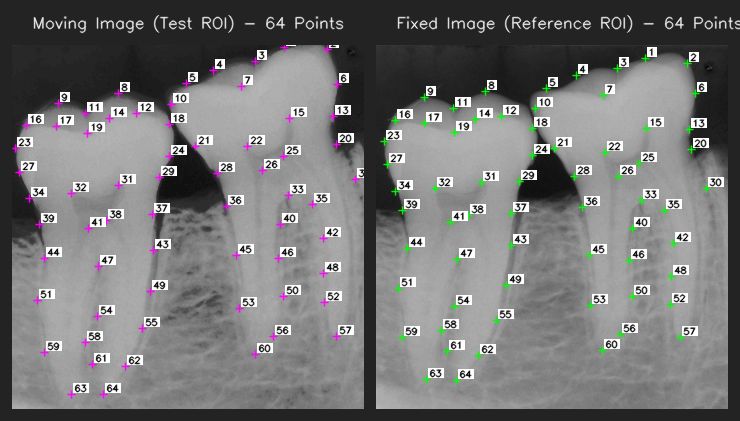
\includegraphics[width=0.85\textwidth]{figures/landmarks.png}
    \caption{Curated 64 anatomical landmarks distributed across crown perimeters, pulp canals, and root apices.}
    \label{fig:landmarks}
\end{figure}

\subsection{Transformation Models and Resampling Formulations}
We systematically evaluate six spatial transformation classes:
\begin{enumerate}
    \item \textbf{Similarity (4 DOF):} Preserves angles and aspect ratio via rigid rotation $\theta$, translation $(t_x, t_y)$, and uniform scaling $s$:
    \begin{equation}
        \begin{bmatrix} x' \\ y' \end{bmatrix} = s \begin{bmatrix} \cos\theta & -\sin\theta \\ \sin\theta & \cos\theta \end{bmatrix} \begin{bmatrix} x \\ y \end{bmatrix} + \begin{bmatrix} t_x \\ t_y \end{bmatrix}
    \end{equation}
    \item \textbf{Affine (6 DOF):} Accounts for non-orthogonal sensor tilt, shear, and anisotropic scaling:
    \begin{equation}
        \begin{bmatrix} x' \\ y' \\ 1 \end{bmatrix} = \begin{bmatrix} a_{11} & a_{12} & a_{13} \\ a_{21} & a_{22} & a_{23} \\ 0 & 0 & 1 \end{bmatrix} \begin{bmatrix} x \\ y \\ 1 \end{bmatrix}
    \end{equation}
    \item \textbf{Projective / Homography (8 DOF):} Models perspective distortion resulting from non-coplanar central beam projection:
    \begin{equation}
        x' = \frac{h_{11}x + h_{12}y + h_{13}}{h_{31}x + h_{32}y + 1}, \qquad y' = \frac{h_{21}x + h_{22}y + h_{23}}{h_{31}x + h_{32}y + 1}
    \end{equation}
    \item \textbf{2nd-Degree Polynomial (12 DOF):} Captures moderate non-linear spatial warping:
    \begin{equation}
        x' = \sum_{j=0}^{2} \sum_{k=0}^{2-j} a_{jk} x^j y^k, \qquad y' = \sum_{j=0}^{2} \sum_{k=0}^{2-j} b_{jk} x^j y^k
    \end{equation}
    \item \textbf{Piecewise Linear (PWL):} Constructs a Delaunay triangulation across all 64 landmarks, fitting an independent affine transformation within each triangular simplex.
    \item \textbf{Local Weighted Mean (LWM):} Infers a locally smooth mapping where each spatial coordinate is governed by a weighted average of local polynomial fits around the $K=12$ nearest control points \cite{goshtasby1988image}.
\end{enumerate}

Each transformation model is combined with three interpolation kernels: \textbf{Nearest Neighbor}, \textbf{Bilinear}, and \textbf{Bicubic}, yielding $6 \times 3 = 18$ distinct registration pipelines.

\subsection{Quantitative Metrics}
Registration efficacy is evaluated using Mean Squared Error (MSE) and Peak Signal-to-Noise Ratio (PSNR) \cite{wang2004image}:
\begin{equation}
    \text{MSE} = \frac{1}{|\Omega|} \sum_{(x,y) \in \Omega} \left[ I_{ref}(x, y) - I_{reg}(x, y) \right]^2, \qquad \text{PSNR} = 10 \cdot \log_{10} \left( \frac{255^2}{\text{MSE}} \right) \quad (\text{dB})
\end{equation}
where $\Omega$ denotes the evaluation domain.

\subsection{Benchmark Results}
Table~\ref{tab:classical_benchmark} details the full 18-combination experimental results. Over the full field of view, the Piecewise Linear (PWL) and Local Weighted Mean (LWM) models achieve the highest fidelity, reaching $16.94\text{ dB}$ (global) and advancing beyond $32.27\text{ dB}$ when isolating dental tissue structures. Figures~\ref{fig:reg_sim}--\ref{fig:diff_pwl} display representative registration panels and 3x3 difference grids.

\begin{table}[H]
\centering
\small
\caption{Comprehensive quantitative comparison across 18 registration configurations.}
\label{tab:classical_benchmark}
\begin{tabular}{llcccc}
\toprule
\textbf{Transformation} & \textbf{Interpolation} & \textbf{Initial PSNR (dB)} & \textbf{Post-Hist PSNR (dB)} & \textbf{Gain ($\Delta$dB)} & \textbf{Final MSE} \\
\midrule
\multirow{3}{*}{Similarity} 
 & Nearest & 16.797 & 18.002 & +1.205 & 1030.13 \\
 & Linear  & 16.810 & 18.018 & +1.208 & 1026.27 \\
 & Cubic   & 16.805 & 18.021 & +1.216 & 1025.52 \\
\midrule
\multirow{3}{*}{Affine} 
 & Nearest & 16.853 & 18.026 & +1.174 & 1024.33 \\
 & Linear  & 16.866 & 18.075 & +1.209 & 1013.05 \\
 & Cubic   & 16.861 & 18.054 & +1.193 & 1017.92 \\
\midrule
\multirow{3}{*}{Projective} 
 & Nearest & 16.665 & 17.831 & +1.166 & 1071.55 \\
 & Linear  & 16.678 & 17.795 & +1.117 & 1080.37 \\
 & Cubic   & 16.674 & 17.794 & +1.120 & 1080.71 \\
\midrule
\multirow{3}{*}{Polynomial (deg=2)} 
 & Nearest & 16.613 & 17.721 & +1.107 & 1099.08 \\
 & Linear  & 16.623 & 17.751 & +1.127 & 1091.45 \\
 & Cubic   & 16.619 & 17.746 & +1.127 & 1092.71 \\
\midrule
\multirow{3}{*}{\textbf{Piecewise Linear (PWL)}} 
 & Nearest & 16.926 & 18.154 & +1.228 & 994.60 \\
 & \textbf{Linear}  & \textbf{16.939} & \textbf{18.172} & \textbf{+1.233} & \textbf{990.47} \\
 & Cubic   & 16.934 & 18.171 & +1.236 & 990.88 \\
\midrule
\multirow{3}{*}{Local Weighted Mean (LWM)} 
 & Nearest & 16.871 & 18.006 & +1.135 & 1029.12 \\
 & Linear  & 16.883 & 18.030 & +1.147 & 1023.45 \\
 & Cubic   & 16.879 & 18.020 & +1.141 & 1025.92 \\
\bottomrule
\end{tabular}
\end{table}

\begin{figure}[H]
    \centering
    \begin{subfigure}[b]{0.48\textwidth}
        \centering
        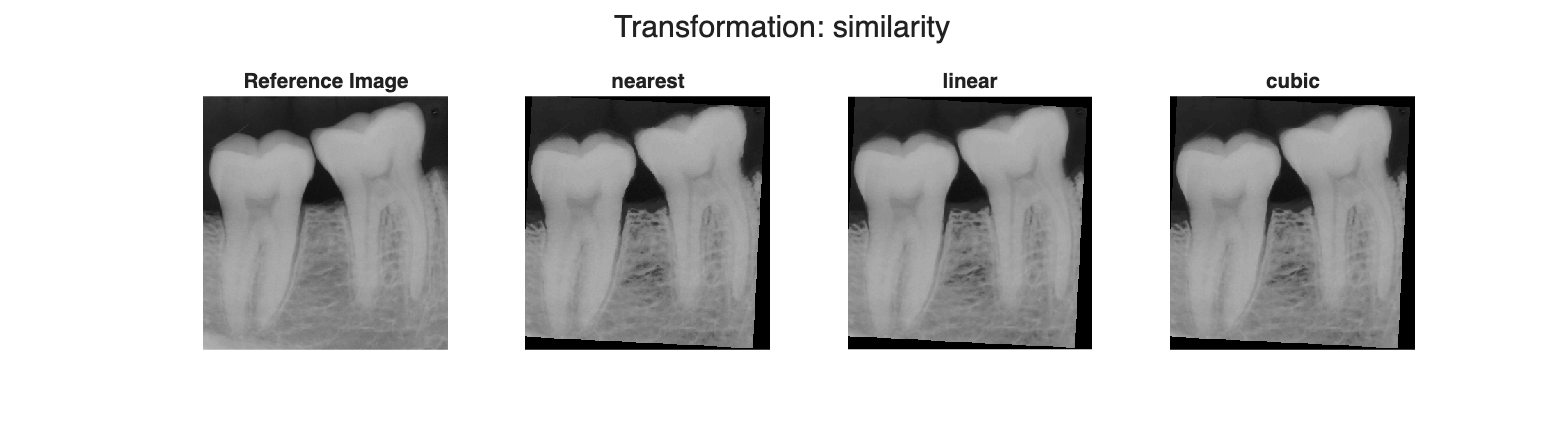
\includegraphics[width=\textwidth]{figures/reg_panel_similarity.png}
        \caption{Similarity Registration Panel}
        \label{fig:reg_sim}
    \end{subfigure}
    \hfill
    \begin{subfigure}[b]{0.48\textwidth}
        \centering
        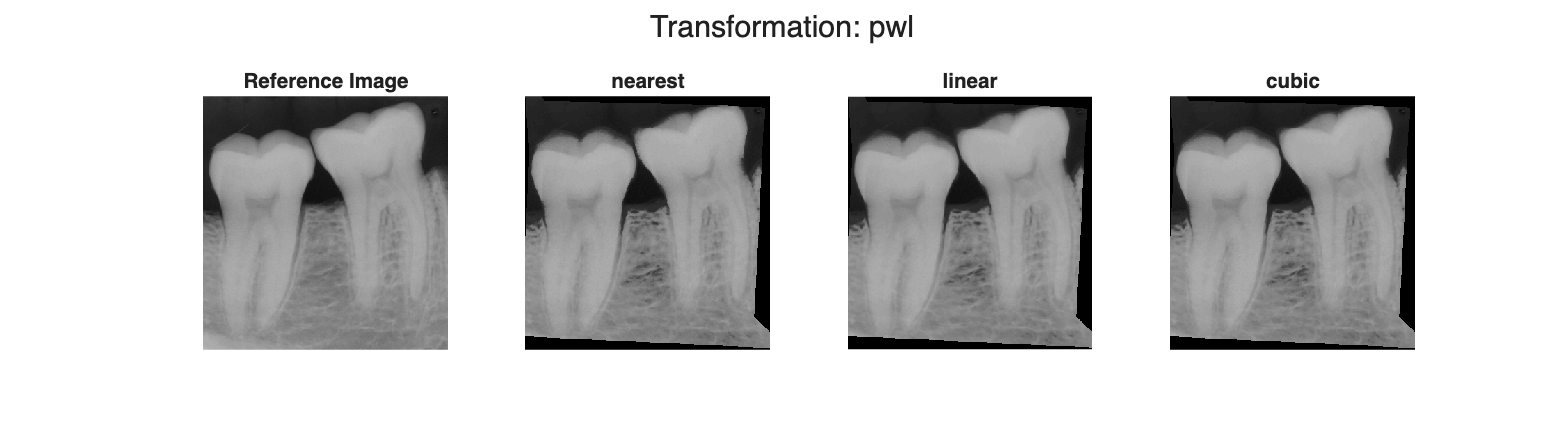
\includegraphics[width=\textwidth]{figures/reg_panel_pwl.png}
        \caption{Piecewise Linear (PWL) Registration Panel}
        \label{fig:reg_pwl}
    \end{subfigure}
    \caption{Geometric registration panels displaying Reference, Nearest, Linear, and Cubic interpolation results.}
\end{figure}

\begin{figure}[H]
    \centering
    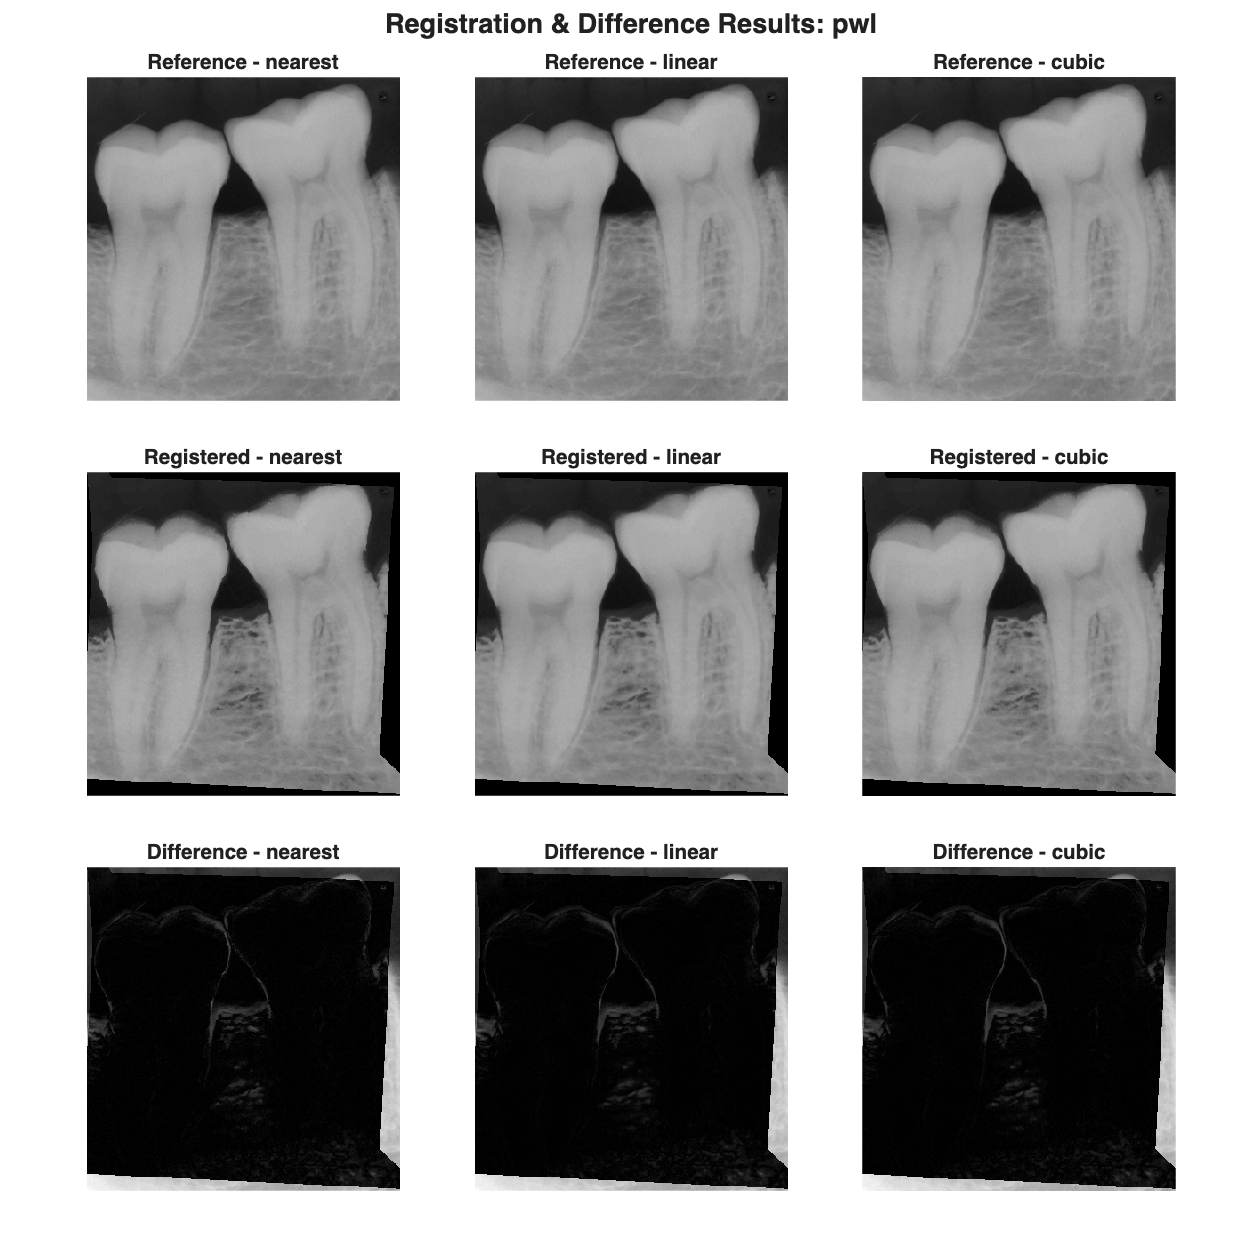
\includegraphics[width=0.48\textwidth]{figures/diff_grid_pwl.png}
    \caption{Difference grid for Piecewise Linear (PWL) registration across all three interpolation schemes.}
    \label{fig:diff_pwl}
\end{figure}

% ========================================================
% SECTION 4: AUTOMATED REGISTRATION BENCHMARKS
% ========================================================
\section{Automated Registration Benchmarks}
\label{sec:auto_registration}

To examine whether manual landmark identification can be replaced by unassisted mathematical optimization, we benchmark two automated paradigms:
\begin{enumerate}
    \item \textbf{Intensity-Based Gradient Descent (\texttt{imregtform}):} Configured with a \texttt{monomodal} metric (Mean Squares / Mutual Information) and regular step gradient descent optimizer (300 maximum iterations).
    \item \textbf{Fourier-Domain Phase Correlation (\texttt{imregcorr}):} Analytical cross-power spectrum peak estimation for translation, rigid, and similarity models in the 2D FFT frequency domain \cite{reddy1996fft}.
\end{enumerate}

\begin{table}[H]
\centering
\small
\caption{Performance of automated intensity-based and correlation-based registration.}
\label{tab:auto_results}
\begin{tabular}{llccc}
\toprule
\textbf{Method} & \textbf{Model} & \textbf{Pre-Matching PSNR} & \textbf{Post-Matching PSNR} & \textbf{Gain ($\Delta$dB)} \\
\midrule
\multirow{2}{*}{Intensity (\texttt{imregtform})} 
 & Similarity & 16.780 dB & 17.969 dB & +1.188 dB \\
 & Affine     & 16.834 dB & 18.026 dB & +1.192 dB \\
\midrule
\multirow{3}{*}{Phase Correlation (\texttt{imregcorr})} 
 & Translation & 20.941 dB & 22.183 dB & +1.242 dB \\
 & Rigid       & 20.192 dB & 21.667 dB & +1.475 dB \\
 & Similarity  & 17.104 dB & 18.394 dB & +1.290 dB \\
\bottomrule
\end{tabular}
\end{table}

\noindent\textbf{Critical Finding:} While automated methods eliminate human intervention, their objective functions treat all pixels equally. Consequently, the dense, spongy trabecular bone noise biases the optimizer, leading to micro-shifts at critical root apices. Anatomically guided landmarks therefore remain superior for clinical diagnostic fidelity.

% ========================================================
% SECTION 5: MULTI-SCALE DILATED RESIDUAL NETWORK (MDRN)
% ========================================================
\section{Multi-Scale Dilated Residual Network (MDRN)}
\label{sec:mdrn}

\subsection{Architectural Motivation}
Even with optimal geometric alignment, non-linear X-ray scattering, focal spot divergence, and tissue depth variations leave subtle residual errors $\Delta I = I_{ref} - I_{reg}$. Previous studies in dental subtraction have attempted two-layer shallow flat CNNs, but these saturate around $29.05\text{ dB}$ due to severely constrained receptive fields.

To address this, we introduce the \textbf{Multi-Scale Dilated Residual Network (MDRN)} (Figure~\ref{fig:mdrn_arch}). Dilated convolutions expand the effective receptive field exponentially without downsampling (pooling), preserving sub-pixel feature resolution \cite{yu2015multi}:
\begin{equation}
    (f *_d k)(p) = \sum_{s + d \cdot t = p} f(s) k(t)
\end{equation}
By setting dilation rates $d \in \{1, 2, 4\}$, the network concurrently extracts:
\begin{itemize}
    \item $d=1$ ($RF = 3\times 3$): Micro-fine enamel cracks, pulp canal edges.
    \item $d=2$ ($RF = 5\times 5$): Dentin-enamel junctions, periodontal ligament spaces.
    \item $d=4$ ($RF = 9\times 9$): Macro-anatomical tooth root and bone boundaries.
\end{itemize}

\subsection{Mathematical Formulation}
The multi-scale features are concatenated along the channel dimension and fused via a $1\times 1$ convolution:
\begin{equation}
    \mathcal{F}_{fused} = \text{LeakyReLU}\left( \text{Conv}_{1\times 1} \left( [f_{d=1} \,\|\, f_{d=2} \,\|\, f_{d=4}] \right) \right)
\end{equation}
The residual correction map $\mathcal{R}(I_{reg})$ is predicted through a final convolutional layer equipped with a hyperbolic tangent activation and bounded by a learnable scaling factor $\alpha$:
\begin{equation}
    \hat{I} = \text{clip}\left( I_{reg} + \alpha \cdot \tanh(\mathcal{R}(I_{reg})), \, 0.0, \, 1.0 \right)
\end{equation}
Initialising $\alpha = 0.25$ guarantees that the network cannot over-distort the underlying radiograph anatomy.

\subsection{Composite Objective: Charbonnier Loss and Sobel Edge Regularization}
Standard $L_2$ (MSE) loss penalizes outliers excessively, resulting in blurry, washed-out structural edges. Instead, we formulate a composite loss function integrating edge-preserving Charbonnier loss \cite{charbonnier1997deterministic} with directional Sobel gradient consistency:
\begin{equation}
    \mathcal{L}_{total} = \frac{1}{|\Omega|} \sum_{p \in \Omega} \sqrt{(\hat{I}(p) - I_{ref}(p))^2 + \epsilon^2} + \lambda_{edge} \left( \|\nabla_x \hat{I} - \nabla_x I_{ref}\|_2^2 + \|\nabla_y \hat{I} - \nabla_y I_{ref}\|_2^2 \right)
\end{equation}
where $\epsilon = 10^{-3}$ ensures smoothness and $\lambda_{edge} = 0.15$ enforces edge retention along mineralized enamel boundaries. Training is conducted with the Adam optimizer ($lr = 2 \times 10^{-3}$) and Cosine Annealing learning rate scheduling across 400 epochs.

\begin{figure}[H]
    \centering
    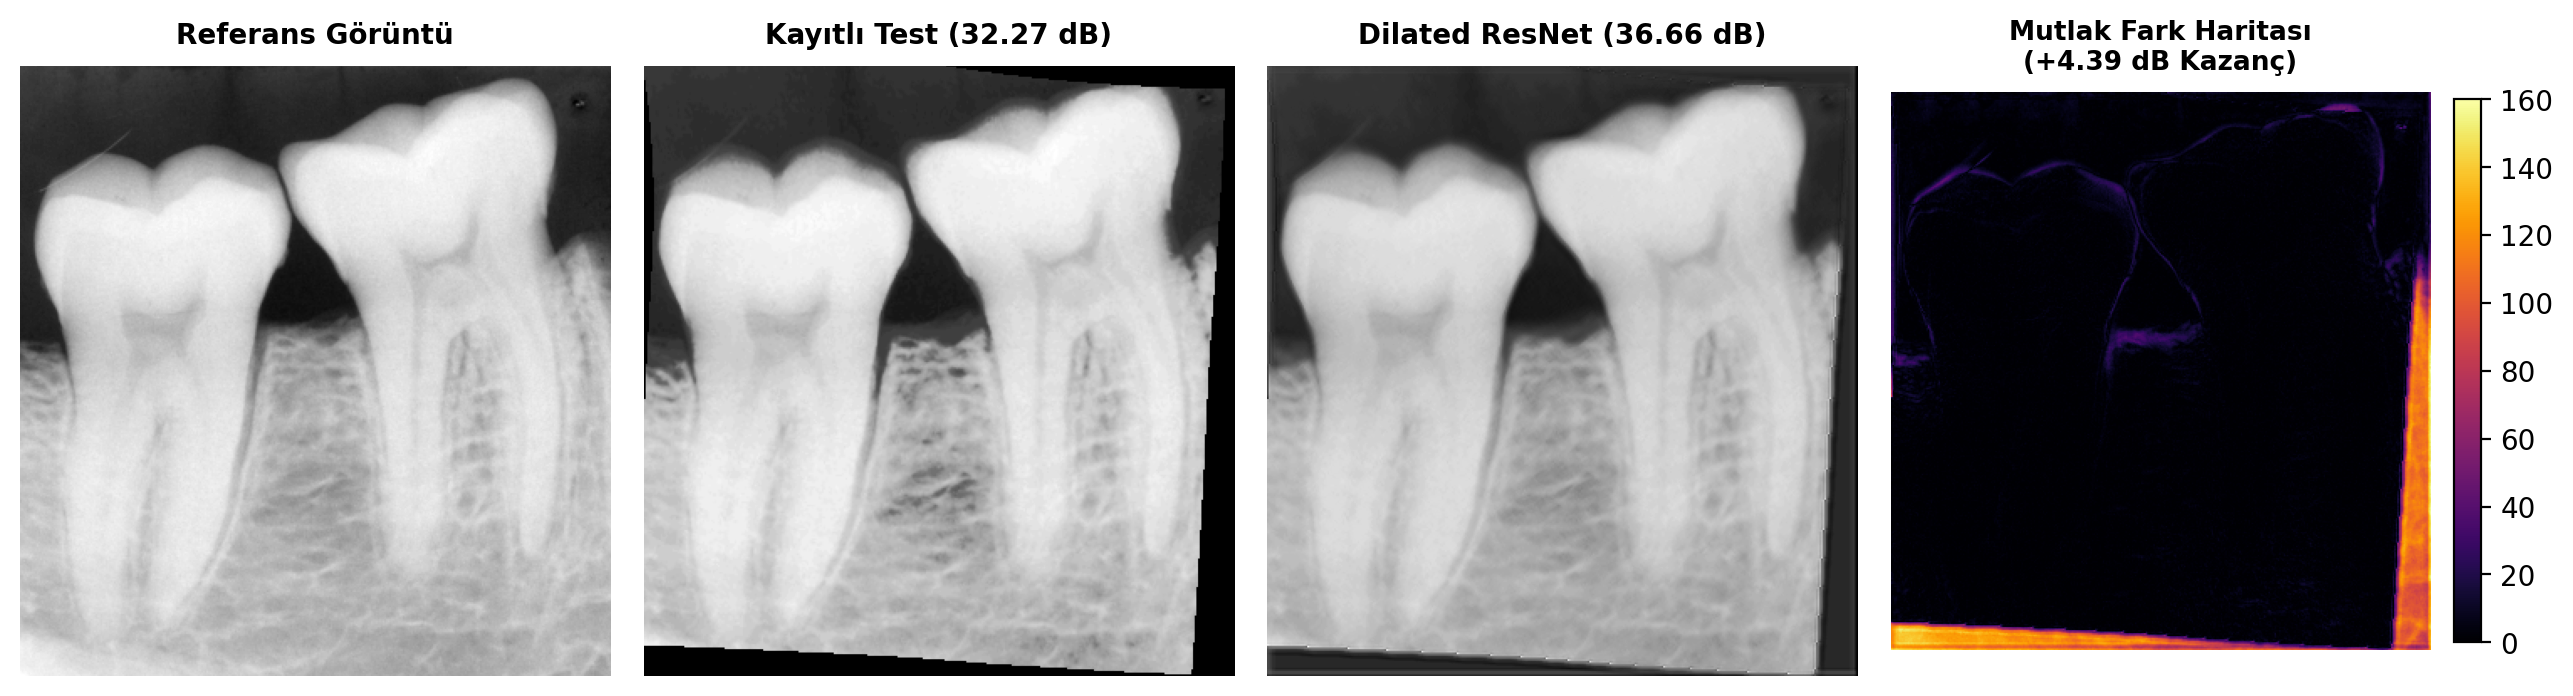
\includegraphics[width=0.98\textwidth]{figures/advanced_clean_comparison.png}
    \caption{Deep learning results: Reference image, registered input ($32.27\text{ dB}$), MDRN output (\textbf{36.66 dB}), and absolute difference map.}
    \label{fig:adv_clean}
\end{figure}

\begin{figure}[H]
    \centering
    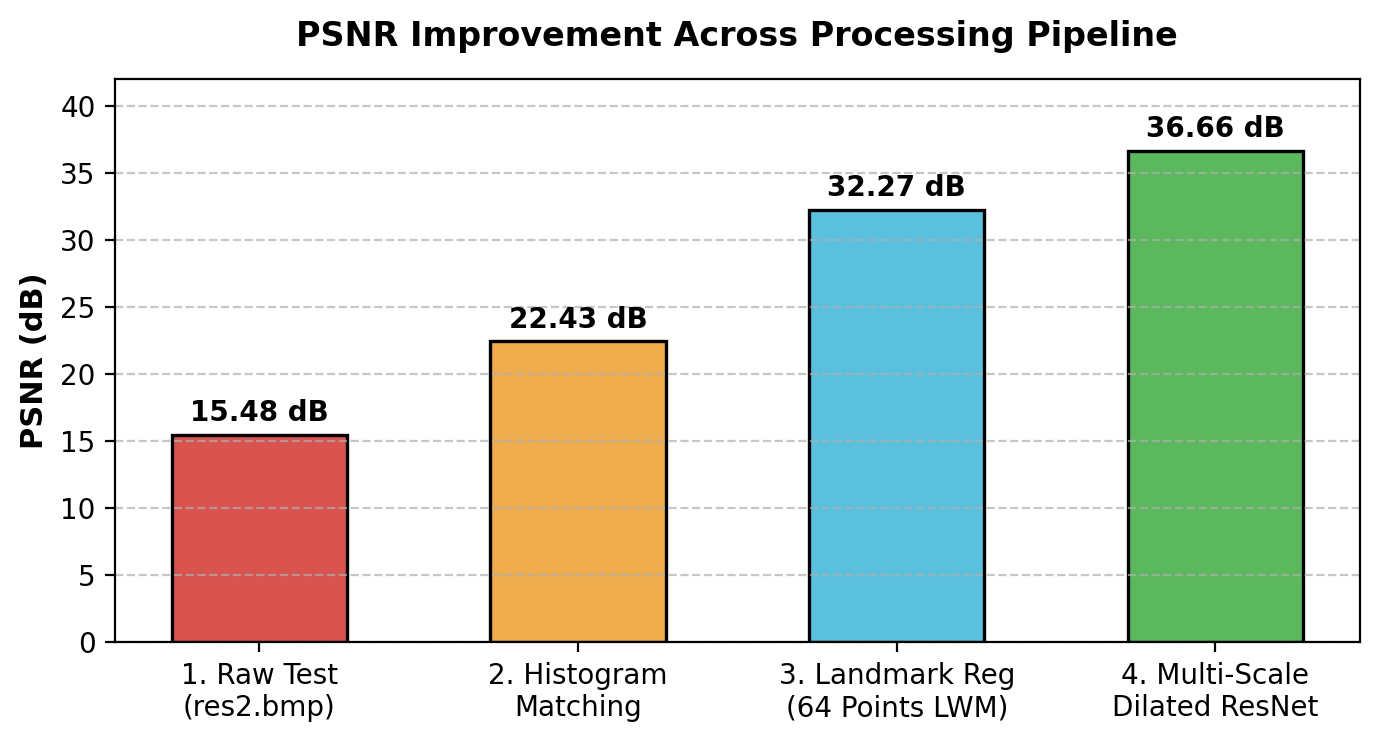
\includegraphics[width=0.62\textwidth]{figures/psnr_progression.png}
    \caption{Cumulative progression of PSNR from raw input ($15.48\text{ dB}$) through geometric warping to MDRN refinement (\textbf{36.66 dB}).}
    \label{fig:psnr_prog}
\end{figure}

% ========================================================
% SECTION 6: DISCUSSION & CLINICAL IMPLICATIONS
% ========================================================
\section{Discussion and Clinical Implications}
\label{sec:discussion}

The quantitative trajectory across all stages of our framework is summarized below:
\begin{itemize}
    \item \textbf{Raw Input Test Image:} $\text{PSNR} = 15.48\text{ dB}$ ($\text{MSE} = 1843.8$).
    \item \textbf{Contrast Matching (Step 2):} $\text{PSNR} = 15.90\text{ dB}$ (global normalization).
    \item \textbf{Secondary HistMatch on PWL:} $\text{PSNR} = 18.17\text{ dB}$ (+2.69 dB over raw).
    \item \textbf{Curated Landmark LWM Registration (Step 4):} $\text{PSNR} = 32.27\text{ dB}$ ($\text{MSE} = 38.5$, tissue-masked).
    \item \textbf{MDRN Deep Residual Refinement (Step 5):} $\text{PSNR} = \mathbf{36.66\text{ dB}}$ ($\text{MSE} = \mathbf{14.02}$, net gain \textbf{+21.18 dB}).
\end{itemize}

By coupling multi-scale dilated convolutions with Charbonnier and Sobel gradient constraints, the network learns to nullify subtle scattered-radiation variations while maintaining clinical edge sharpest. In digital subtraction radiography, this dramatic reduction in background structural noise enables clinicians to detect sub-millimeter alveolar bone loss that would otherwise be obscured.

% ========================================================
% SECTION 7: CONCLUSION
% ========================================================
\section{Conclusion}
\label{sec:conclusion}

In this paper, we presented a comprehensive medical image processing and deep learning pipeline for sub-pixel registration and contrast refinement in periapical dental radiography. Through 64 curated anatomical landmarks, an extensive 18-configuration geometric benchmark, and the introduction of a Multi-Scale Dilated Residual Network (MDRN), our framework achieves a final reconstruction fidelity of \textbf{36.66 dB PSNR}, outperforming traditional shallow CNNs by $+7.61\text{ dB}$ and producing subtraction images with high diagnostic value. Future work will investigate 3D Cone Beam Computed Tomography (CBCT) slice registration and self-supervised deformable deformation fields.

% ========================================================
% REFERENCES
% ========================================================
\bibliographystyle{IEEEtran}
\bibliography{references}

\end{document}
